\chapter{LAB 01: Introduction to OS161 and the Build System}

\section{The Nature of OS161 and Sys161}
Operating systems are inherently complex software constructs, often spanning millions of lines of code, making them overwhelmingly difficult to study and modify in a purely theoretical or real-world hardware context. 

OS161 was specifically designed at Harvard University to circumvent this complexity. It is an instructional, Unix BSD-like operating system written in C that prioritizes code readability and pedagogical value over raw performance. 

It provides a foundational layer including low-level trap and interrupt handling, device drivers, in-kernel threads, a baseline scheduler, a minimal virtual memory system, and a rudimentary file system. By working with OS161, we gain a hands-on, realistic environment to practice operating system development without being bogged down by legacy hardware quirks.

\subsection{What is an Emulator?}
To ensure a consistent, safe, and easily debuggable hardware experience, OS161 does not run on "bare metal" (the physical hardware of your laptop). Instead, it is executed atop a virtual machine known as \textbf{sys161}. 

An emulator is a specialized software application that perfectly mimics the internal architecture of a specific physical CPU and its peripheral devices. Sys161 specifically simulates a \textbf{MIPS R3000 microprocessor}. The MIPS architecture was chosen because its Reduced Instruction Set Computer (RISC) design is clean, elegant, and highly educational, completely avoiding the historical and structural complexities associated with architectures like x86. 

It is crucial to distinguish between the two distinct entities: 
\begin{itemize}
    \item \texttt{sys161} is the \textbf{emulator software}. It runs natively on your host machine (e.g., Linux or macOS). It provides the fake CPU, fake RAM, and fake hard drives.
    \item \texttt{os161} is the \textbf{actual operating system code}. When compiled, it becomes a binary executable (e.g., \texttt{kernel-DUMBVM}). 
\end{itemize}
When the command \texttt{sys161 kernel} is executed, the emulator boots up the simulated MIPS machine and loads your compiled OS executable into its simulated RAM, just like a real motherboard loading an OS from a hard drive.

\subsection{Cross-Compilation Explained}
Because your host machine (likely an x86\_64 or ARM Mac/PC) has a fundamentally different architecture than the target machine (MIPS), you cannot use your system's default \texttt{gcc} compiler to build the OS161 kernel. If you did, it would generate x86/ARM machine code, which the MIPS emulator cannot understand.

This necessitates \textbf{cross-compilation}. Cross-compilation is the process of building executable code for a platform other than the one on which the compiler is running. The OS161 toolchain includes a specially built version of GCC (\texttt{mips-harvard-os161-gcc}). When you compile your C code using this specific compiler, it runs on your host machine but translates the C code directly into MIPS assembly and MIPS machine code.

\section{Project Structure Overview}
Understanding where files are located is paramount before modifying the kernel. Imagine the OS161 project as being split into three major domains: the cross-compilation tools, the source code, and the deployment root.

\begin{verbatim}
os161/
|-- tools/                 # The cross-compilation toolchain (MIPS GCC, GDB, bmake, sys161)
|-- os161-base-2.0.2/      # The actual source code of the operating system
|   |-- kern/              # 1. KERNEL SOURCE CODE (Where you will work)
|   |   |-- arch/mips/     # Low-level MIPS architecture code (traps, assembly)
|   |   |-- compile/       # Build directories generated by ./config
|   |   |-- conf/          # Configuration files (conf.kern, DUMBVM)
|   |   |-- include/       # Kernel header files (.h)
|   |   |-- main/          # Kernel entry point (main.c)
|   |   |-- proc/          # Process management code (proc.c)
|   |   |-- syscall/       # System call implementations (you will create file_syscalls.c)
|   |   |-- thread/        # Thread management and synchronization (synch.c)
|   |   |__ vm/            # Virtual memory implementation (dumbvm.c)
|   |__ userland/          # 2. USER-SPACE PROGRAMS (C standard library, test binaries)
|__ root/                  # 3. THE SIMULATED HARD DRIVE
                           # This is where the compiled kernel and user binaries are 
                           # installed. Sys161 boots from this folder.
\end{verbatim}

\section{The OS161 Build System}
Building the OS161 kernel involves a strict, sequential four-step pipeline managed by BSD make (\texttt{bmake}).

\subsection{1. Configuring the Kernel (\texttt{./config})}
Before any compilation can occur, the build tree must be generated. This is achieved by navigating to the \texttt{kern/conf} directory and executing \texttt{./config DUMBVM} (or your specific configuration name). 
The \texttt{config} script reads the master \texttt{conf.kern} file (which defines all possible options and files) and the specific \texttt{DUMBVM} file (which selects which options to activate). It then generates a dedicated compile directory (\texttt{kern/compile/DUMBVM}) populated with the necessary Makefiles and auto-generated headers.

\subsection{2. Building the Dependency Graph (\texttt{bmake depend})}
Once configured, we navigate to the generated compile directory (\texttt{kern/compile/DUMBVM}) and execute \texttt{bmake depend}. 
This crucial step invokes the C preprocessor to scan all source files for \texttt{\#include} directives. It builds a comprehensive dependency graph (mapping which \texttt{.c} files rely on which \texttt{.h} files). This ensures that during subsequent rebuilds, if you modify a single header file, \texttt{bmake} knows exactly which source files need to be recompiled, saving immense amounts of time.

\subsection{3. Compilation and Linking (\texttt{bmake})}
Running \texttt{bmake} performs the actual cross-compilation. It translates the C source code into MIPS object files (\texttt{.o}) and links them together to generate the final binary executable named \texttt{kernel-DUMBVM}.

\subsection{4. Installation (\texttt{bmake install})}
Compiling alone is insufficient. The \texttt{kernel-DUMBVM} executable currently sits in the compile directory. The emulator, however, is configured to boot from the \texttt{root} directory. The command \texttt{bmake install} copies the newly generated executable into the \texttt{root} directory and updates a symbolic link named \texttt{kernel} to point to it, ensuring the emulator boots the fresh kernel rather than a stale version.

\subsection{VSCode Build and Debug Integration}
While the traditional terminal workflow is fundamental to understanding the build system, modern development often utilizes IDEs. A correctly configured Visual Studio Code environment maps these terminal commands to VSCode Tasks:
\begin{itemize}
    \item \textbf{Terminal $\rightarrow$ Run Task $\rightarrow$ Run Config}: Maps to \texttt{./config}. You select the configuration (e.g., \texttt{HELLO}, \texttt{DUMBVM}) and it generates the \texttt{kern/compile/} directory.
    \item \textbf{Terminal $\rightarrow$ Run Task $\rightarrow$ Make depend}: Maps to \texttt{bmake depend}.
    \item \textbf{Terminal $\rightarrow$ Run Task $\rightarrow$ Build and Install}: Maps to \texttt{bmake} followed by \texttt{bmake install}.
\end{itemize}

For debugging directly in VSCode:
\begin{enumerate}
    \item Execute \textbf{Terminal $\rightarrow$ Run Task $\rightarrow$ RUN OS161}. This starts the simulator in listening mode (\texttt{sys161 -w kernel}).
    \item Execute \textbf{Run $\rightarrow$ Start Debugging}. This attaches the GDB debugger.
    \item You can now set breakpoints visually (e.g., inside \texttt{kmain}) and step through the code.
\end{enumerate}

\section{Adding a Custom Boot Message (Configuration Deep Dive)}
A core exercise in this laboratory demonstrates the modular nature of the OS161 build system by adding a custom "Hello" message during the boot sequence. This introduces the concept of \textbf{Kernel Configuration Options}.

When you modify the master configuration file \texttt{kern/conf/conf.kern}, you define new features:
\begin{lstlisting}[language=C]
// In kern/conf/conf.kern
defoption hello
optfile hello main/hello.c
\end{lstlisting}

\textbf{How it works:}
\begin{itemize}
    \item \texttt{defoption hello}: This tells the build system that an option named "hello" exists. During the \texttt{./config} step, the script will \textit{always} auto-generate a header file named \texttt{opt-hello.h}. If the option is enabled in the specific configuration file (e.g., \texttt{DUMBVM}), the header will contain \texttt{\#define OPT\_HELLO 1}. If it is disabled or absent, the header will contain \texttt{\#define OPT\_HELLO 0}.
    \item \texttt{optfile hello main/hello.c}: This tells the build system that the source file \texttt{main/hello.c} should \textit{only} be compiled and linked into the final kernel if the "hello" option is enabled.
\end{itemize}

We then provide the implementation by creating \texttt{hello.h} and \texttt{hello.c}.
\begin{lstlisting}[language=C]
// In kern/main/hello.c
#include <types.h>
#include <lib.h>
#include "hello.h"

void hello(void) {
    kprintf("Hello from the new OS161 branch!\n");
}
\end{lstlisting}

To execute this function during boot, we integrate it into the main kernel initialization routine located in \texttt{kern/main/main.c}. It is critical to wrap both the function call and its include directive in a preprocessor conditional checking the auto-generated macro.

\begin{lstlisting}[language=C]
// In kern/main/main.c
#include "opt-hello.h" // ALWAYS included

#if OPT_HELLO
#include "hello.h"     // Included ONLY if OPT_HELLO is 1
#endif

void kmain(char *arguments) {
    boot();
    
#if OPT_HELLO
    hello();           // Executed ONLY if OPT_HELLO is 1
#endif
    
    menu(arguments);
}
\end{lstlisting}

By wrapping the call in \texttt{\#if OPT\_HELLO}, we ensure that if the configuration is disabled, the compiler ignores the block. If we didn't use this \texttt{\#if} check, disabling the option would prevent \texttt{hello.c} from being compiled, leading to a fatal Linker Error because \texttt{kmain} would be trying to call an undefined \texttt{hello()} function.

\subsection*{The \texttt{\#ifdef} vs \texttt{\#if} Trap}
A very common pitfall (and a frequent exam question) is attempting to use \texttt{\#ifdef OPT\_HELLO} instead of \texttt{\#if OPT\_HELLO}. 

In C, \texttt{\#ifdef} checks whether a macro is \textit{defined at all}, regardless of its actual value. As we established earlier, the \texttt{./config} script \textbf{always} generates the \texttt{opt-hello.h} file, and it \textbf{always} defines the macro. 
\begin{itemize}
    \item If enabled: \texttt{\#define OPT\_HELLO 1}
    \item If disabled: \texttt{\#define OPT\_HELLO 0}
\end{itemize}
Because the macro is always defined, \texttt{\#ifdef OPT\_HELLO} will \textbf{always evaluate to TRUE}. If the option was disabled in your configuration, the compiler will attempt to compile the \texttt{hello()} function call anyway. But since \texttt{hello.c} wasn't compiled, the linker will throw a fatal undefined reference error. 

Therefore, you must strictly use \texttt{\#if OPT\_HELLO}, which checks the \textit{mathematical value} of the macro (1 or 0).

\section{Distributed Kernel Debugging}
Debugging an operating system kernel presents unique challenges. You cannot simply run a debugger \textit{inside} an OS that is currently crashing. OS161 utilizes a \textbf{distributed debugging model}. 

\begin{itemize}
    \item \textbf{The Target:} The emulator is started with a flag instructing it to pause and wait for a debugger connection: \texttt{sys161 -w kernel}. This opens a local UNIX domain socket and freezes the simulated CPU before the very first instruction is executed.
    \item \textbf{The Host:} In a separate terminal, the cross-compiled debugger is launched: \texttt{mips-harvard-os161-gdb kernel}. 
    \item \textbf{The Connection:} Within GDB, the command \texttt{target remote unix:.sockets/gdb} establishes the connection to the paused emulator, allowing for breakpoints, stepping, and state inspection over the socket.
\end{itemize}

When debugging concurrent threads (e.g., during \texttt{thread\_fork}), special care must be taken. Stepping \textit{over} a fork instruction keeps the debugger attached to the parent thread, while the newly spawned thread executes freely in the background. To debug the child thread, a breakpoint must be explicitly set on its entry function before allowing the parent to continue execution.

\section{Core OS161 Data Types: \texttt{vaddr\_t} vs \texttt{paddr\_t}}
When working with kernel memory, it is vital to distinguish between virtual and physical addresses. 

\begin{itemize}
    \item \textbf{\texttt{paddr\_t} (Physical Address):} Represents an actual, hardware-level address in the physical RAM. It is strictly managed by the kernel and cannot be accessed directly by user processes. It is used when interfacing with low-level hardware structures or during manual memory mapping.
    \item \textbf{\texttt{vaddr\_t} (Virtual Address):} Represents the address as seen by a process or by the kernel itself. 
\end{itemize}

Every process operates within its own isolated virtual address space. When a process attempts to access a \texttt{vaddr\_t}, the Memory Management Unit (MMU) translates it to a corresponding \texttt{paddr\_t} using a Page Table. This abstraction means that the exact same \texttt{vaddr\_t} in Process A and Process B will translate to entirely different \texttt{paddr\_t} physical locations.

\begin{figure}[h]
    \centering
    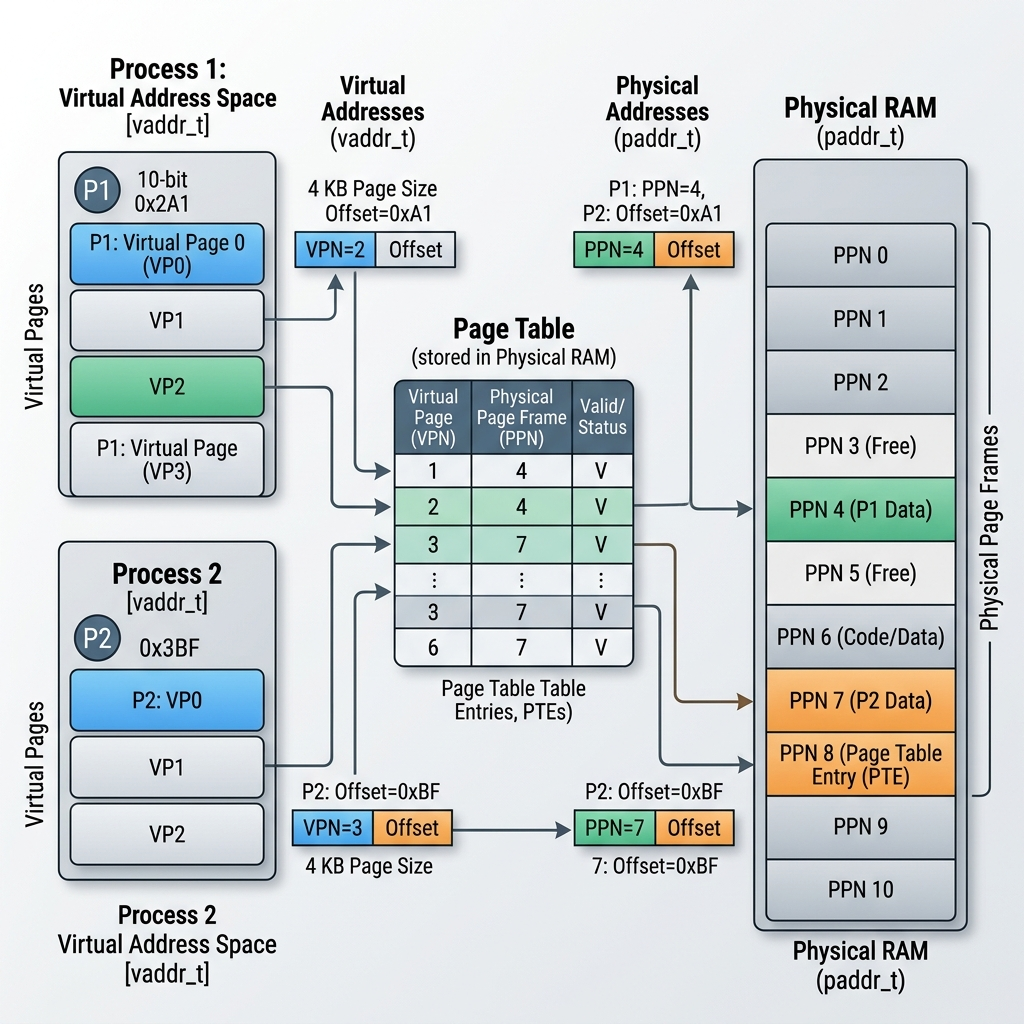
\includegraphics[width=0.8\textwidth]{images/vaddr_to_paddr_mapping.png}
    \caption{Mapping Virtual Addresses (\texttt{vaddr\_t}) to Physical Addresses (\texttt{paddr\_t}).}
\end{figure}

\section{Introduction to OS161 Concurrency}

\subsection{Processes vs Threads}
A \textbf{program} is a passive entity on disk. When it is executed, it becomes a \textbf{process}---an active entity containing executable code, a data section, a heap, an execution stack, and a Program Counter (PC).

A \textbf{thread} is a single flow of execution within a process. A process can contain multiple threads that share the same code, global data, and open files, but each thread maintains its own:
\begin{itemize}
    \item Program Counter (PC)
    \item CPU Register state
    \item Execution Stack
\end{itemize}

OS161 primarily manages \textbf{kernel threads}. The kernel maintains an array or list of thread structures. When a thread is suspended, its execution context (registers and PC) is saved into a \texttt{switchframe} on its stack.

\subsection{The Thread API}
The OS161 thread management library relies on a \texttt{struct thread} containing the thread's name, synchronization primitives, state, stack pointer, and a pointer to its parent process's Process Control Block (PCB).

Key functions include:
\begin{itemize}
    \item \texttt{thread\_fork()}: Creates a new thread. It allocates a new \texttt{struct thread}, initializes the \texttt{switchframe} with \texttt{switchframe\_init()}, and places the thread into the ready queue using \texttt{thread\_make\_runnable()}.
    \item \texttt{thread\_yield()}: Voluntarily suspends the currently running thread, yielding the CPU. It places the thread back in the ready queue (\texttt{S\_READY}) and calls \texttt{thread\_switch()} to execute the next thread.
    \item \texttt{thread\_exit()}: Terminates the current thread.
    \item \texttt{thread\_switch()}: Performs the low-level context switch by swapping the \texttt{switchframe} of the current thread with the next one.
\end{itemize}

\subsection{Testing and Debugging Threads}
OS161 provides built-in commands to test thread concurrency from the kernel menu:
\begin{itemize}
    \item \texttt{tt1}: Creates \texttt{NTHREADS} (usually 8) and runs them in "quiet" mode, where each thread prints a single identifying character.
    \item \texttt{tt2}: Similar to \texttt{tt1}, but runs in "loud" mode, printing the character 120 times. 
    \item \texttt{tt3}: A complex test involving thread synchronization. It uses two sets of threads---one that sleeps for random intervals, and another that performs matrix math.
\end{itemize}

Because threads are scheduled concurrently by the kernel (via \texttt{hardclock} interrupts calling \texttt{thread\_yield}), their execution order is non-deterministic. Threads 0 through 7 will not execute in sequential order.

When debugging threads using GDB, setting breakpoints on \texttt{thread\_create}, \texttt{thread\_fork}, \texttt{thread\_yield}, and \texttt{thread\_switch} allows you to trace the lifecycle and context switching of these concurrent execution flows.

\newpage

\section{Laboratory 01: Print hello world in OS161}

\subsection{High-Level Overview}
The primary objective of Laboratory 01 is to familiarize yourself with the OS161 build system and the kernel configuration process. Instead of modifying core OS mechanics, you will implement a custom modular feature: a greeting message that prints during the kernel boot sequence.

To achieve this safely without breaking the build, you must follow the strict OS161 pipeline:
\begin{enumerate}
    \item Define a new kernel option (\texttt{hello}) in the master configuration file.
    \item Enable the option for your specific kernel build.
    \item Create the actual C source code and header file for the greeting.
    \item Integrate the function call safely into the kernel's main boot routine.
    \item Reconfigure the build system to generate new headers and Makefiles.
    \item Cross-compile and deploy the modified kernel to the simulated MIPS hardware.
\end{enumerate}

\subsection{Step 1: Define the Option in \texttt{conf.kern}}
First, we must tell the OS161 build system that a new optional feature exists and associate it with a source file.
\begin{itemize}
    \item \textbf{Action:} Open the master configuration file at \texttt{kern/conf/conf.kern}.
    \item \textbf{Addition:} Scroll to the very bottom and add the following lines:
\begin{lstlisting}[language=C]
defoption hello
optfile hello main/hello.c
\end{lstlisting}
    \item \textbf{Why it is needed:} \texttt{defoption hello} ensures the \texttt{./config} script generates the \texttt{opt-hello.h} macro file. \texttt{optfile} tells the compiler that the file \texttt{hello.c} belongs to this option and should only be compiled if the option is activated.
\end{itemize}

\subsection{Step 2: Enable the Option in \texttt{DUMBVM}}
Defining the option doesn't activate it. We must explicitly turn it on for our specific kernel build.
\begin{itemize}
    \item \textbf{Action:} Open your target configuration file at \texttt{kern/conf/DUMBVM}.
    \item \textbf{Addition:} Add the following line at the bottom:
\begin{lstlisting}[language=C]
options hello
\end{lstlisting}
    \item \textbf{Why it is needed:} This line instructs the configuration script to set the auto-generated macro \texttt{OPT\_HELLO} to \texttt{1} instead of \texttt{0}, effectively enabling the feature.
\end{itemize}

\subsection{Step 3: Create the Source Code and Header File}
Now we write the actual logic for the greeting.
\begin{itemize}
    \item \textbf{Action:} Create a new header file \texttt{kern/include/hello.h} and define the function blueprint:
\begin{lstlisting}[language=C]
#ifndef _HELLO_H_
#define _HELLO_H_

void hello(void);

#endif /* _HELLO_H_ */
\end{lstlisting}
    \item \textbf{Action:} Create a new source file \texttt{kern/main/hello.c} and implement the function:
\begin{lstlisting}[language=C]
#include <types.h>
#include <lib.h>
#include "hello.h"

void hello(void) {
    kprintf("Hello from the new OS161 branch!\n");
}
\end{lstlisting}
    \item \textbf{Why it is needed:} Separating prototypes (\texttt{.h}) from implementations (\texttt{.c}) is a strict requirement in C and OS161 to satisfy the compiler's \texttt{-Wmissing-prototypes} safety flag.
\end{itemize}

\subsection{Step 4: Integrate into the Boot Sequence}
The kernel must actually execute your function when it boots up.
\begin{itemize}
    \item \textbf{Action:} Open the main kernel file at \texttt{kern/main/main.c}.
    \item \textbf{Addition (Top):} Add the includes near the top of the file, alongside the other includes:
\begin{lstlisting}[language=C]
#include "opt-hello.h"

#if OPT_HELLO
#include "hello.h"
#endif
\end{lstlisting}
    \item \textbf{Addition (Inside \texttt{kmain}):} Locate the \texttt{kmain(char *arguments)} function. Add your call right after \texttt{boot();} and before \texttt{menu(arguments);}:
\begin{lstlisting}[language=C]
#if OPT_HELLO
    hello();
#endif
\end{lstlisting}
    \item \textbf{Why it is needed:} The \texttt{\#if OPT\_HELLO} wrapper ensures your code is safely ignored by the compiler if you ever decide to disable the \texttt{hello} option. Without it, disabling the option would cause a fatal linker error.
\end{itemize}

\subsection{Step 5: Reconfigure the Build System}
Because we added new configuration flags and created new files, the internal Makefiles must be regenerated.
\begin{itemize}
    \item \textbf{Action:} Open your terminal, navigate to the configuration directory, and run the script:
\begin{verbatim}
cd ~/os161/os161-base-2.0.3/kern/conf
./config DUMBVM
\end{verbatim}
    \item \textbf{Why it is needed:} This parses your \texttt{DUMBVM} file and generates the crucial \texttt{opt-hello.h} header file, injecting it into your compile directory.
\end{itemize}

\subsection{Step 6: Compile and Install}
Now we translate the C code into MIPS machine code.
\begin{itemize}
    \item \textbf{Action:} Navigate to the compilation directory and run the build sequence:
\begin{verbatim}
cd ../compile/DUMBVM
bmake depend
bmake
bmake install
\end{verbatim}
    \item \textbf{Why it is needed:} 
    \begin{itemize}
        \item \texttt{bmake depend} maps the relationships of your new \texttt{hello.h} file.
        \item \texttt{bmake} performs the actual cross-compilation into a MIPS executable. 
        \item \texttt{bmake install} moves the resulting \texttt{kernel} binary into the \texttt{~/os161/root} directory so the emulator can find it.
    \end{itemize}
\end{itemize}

\subsection{Step 7: Boot the Simulator}
Finally, verify that your implementation was successful.
\begin{itemize}
    \item \textbf{Action:} Navigate to the root directory and start the OS:
\begin{verbatim}
cd ~/os161/root
sys161 kernel
\end{verbatim}
    \item \textbf{Why it is needed:} The simulator will execute the kernel, and you should now see your custom greeting printed directly to the terminal right before the OS161 menu prompt appears!
\end{itemize}

\newpage

\section*{Configuration and Build Flowchart}
To summarize the entire process of configuring and compiling the OS161 kernel, the following flowchart illustrates the workflow. It shows what happens when \texttt{./config} is executed, how the configuration options are translated into C macros, and the subsequent compilation steps.

\tikzstyle{startstop} = [rectangle, rounded corners, minimum width=3cm, minimum height=1cm,text centered, draw=orange, fill=orange!10]
\tikzstyle{io} = [trapezium, trapezium left angle=70, trapezium right angle=110, minimum width=3cm, minimum height=1cm, text centered, draw=green!60!black, fill=green!10]
\tikzstyle{process} = [rectangle, minimum width=3cm, minimum height=1cm, text centered, draw=blue, fill=blue!10]
\tikzstyle{decision} = [diamond, aspect=2.5, minimum width=3cm, minimum height=1cm, text centered, draw=purple, fill=purple!10]
\tikzstyle{arrow} = [thick,->,>=stealth]

\begin{figure}[htbp]
\centering
\begin{tikzpicture}[node distance=2cm]
\node (start) [startstop] {Edit \texttt{kern/conf/conf.kern}};
\node (config) [io, below of=start] {Run \texttt{./config PROJECT}};
\node (dec1) [decision, below of=config, yshift=-0.5cm] {\texttt{options project} present?};
\node (yes) [process, right of=dec1, xshift=3.5cm] {\texttt{\#define OPT\_PROJECT 1}};
\node (no) [process, left of=dec1, xshift=-3.5cm] {\texttt{\#define OPT\_PROJECT 0}};
\node (depend) [io, below of=dec1, yshift=-1.5cm] {Run \texttt{bmake depend}};
\node (make) [io, below of=depend] {Run \texttt{bmake}};
\node (install) [io, below of=make] {Run \texttt{bmake install}};
\node (end) [startstop, below of=install] {Kernel Ready for Simulator};

\draw [arrow] (start) -- (config);
\draw [arrow] (config) -- (dec1);
\draw [arrow] (dec1) -- node[anchor=south] {Yes (V)} (yes);
\draw [arrow] (dec1) -- node[anchor=south] {No (F)} (no);
\draw [arrow] (yes) |- (depend);
\draw [arrow] (no) |- (depend);
\draw [arrow] (depend) -- (make);
\draw [arrow] (make) -- (install);
\draw [arrow] (install) -- (end);
\end{tikzpicture}
\caption{OS161 Kernel Configuration and Build Workflow}
\end{figure}

\section*{Past Exam Questions}

\textbf{[Exam General - Q1] Describe the significance of the \texttt{bmake depend} step in the compilation pipeline. Why is it necessary, and what happens if it is omitted when a header file is modified?}

\textbf{Answer:} 
The \texttt{bmake depend} command invokes the compiler's preprocessor to scan all C source files for \texttt{\#include} directives. Its purpose is to construct a comprehensive dependency graph mapping which \texttt{.c} files rely on which \texttt{.h} header files. 

It is necessary for optimizing the build process. When \texttt{bmake} is subsequently run, it uses this graph to recompile \textit{only} the \texttt{.c} files that depend on recently modified headers, rather than recompiling the entire millions of lines of OS code.

If \texttt{bmake depend} is omitted after modifying a header file (e.g., changing a struct definition or a function prototype), the build system remains unaware of the structural change. Consequently, \texttt{bmake} will skip recompiling the source files that include that header. This results in a mismatched kernel binary where different modules are compiled with conflicting definitions of memory structures, inevitably causing catastrophic memory corruption, undefined behavior, or kernel panics during runtime.

\vspace{1em}

\textbf{[Exam 2025/01/13 - Q6] Configurazione File in OS161 (Configurazione del Kernel e Compile)}

\textit{È dato un Sistema OS161. Si supponga di aver aggiunto le istruzioni seguenti a \texttt{kern/conf/conf.kern}:}
\begin{verbatim}
defoption project
optfile project syscall/project.c
\end{verbatim}
\textit{e di aver creato il file \texttt{PROJECT} in \texttt{kern/conf}, copiato dal file \texttt{DUMBVM}.}

\textbf{A) Si dica se le azioni descritte, più l’esecuzione (in \texttt{kern/conf}) di \texttt{./config PROJECT}, sono sufficienti affinché il file opzionale \texttt{syscall/project.c} sia compilato quando si eseguono (in \texttt{kern/compile/PROJECT}) i comandi \texttt{bmake depend} e \texttt{bmake}.}

\textbf{Answer:} 
No, non sono sufficienti. Le istruzioni in \texttt{conf.kern} si limitano a *definire* l'esistenza di una nuova opzione chiamata \texttt{project} e ad associarvi il file sorgente \texttt{project.c}. Tuttavia, per far sì che il file venga effettivamente compilato, l'opzione deve essere esplicitamente *attivata* nel file di configurazione specifico del kernel. È strettamente necessario aggiungere la riga \texttt{options project} all'interno del file \texttt{kern/conf/PROJECT} *prima* di eseguire il comando \texttt{./config PROJECT}. Senza questa riga, l'opzione è considerata disabilitata e il build system ignorerà il file sorgente.

\textbf{B) Quale file, tra \texttt{project.h} e \texttt{opt-project.h} viene generato automaticamente dal comando \texttt{./config PROJECT}? Il file viene sempre generato, oppure solo se l’istruzione \texttt{options project} compare nel file \texttt{PROJECT}?}

\textbf{Answer:} 
Il comando \texttt{./config PROJECT} genera automaticamente \textit{solo} il file header \texttt{opt-project.h}. Questo file viene \textbf{sempre} generato, in ogni caso, indipendentemente dal fatto che l'istruzione \texttt{options project} sia presente (attivata) o assente (disattivata) nel file \texttt{PROJECT}. Il file \texttt{project.h} (che conterrebbe le firme delle funzioni come \texttt{project\_init}) NON viene mai generato automaticamente; deve essere scritto manualmente dallo sviluppatore e posizionato nella cartella \texttt{kern/include/}.

\textbf{C) Cosa contiene il file (quello generato automaticamente, citato nella domanda precedente)?}

\textbf{Answer:} 
Il file \texttt{opt-project.h} contiene esclusivamente una macro del pre-processore in linguaggio C. 
\begin{itemize}
    \item Se l'opzione è stata attivata inserendo \texttt{options project} nel file \texttt{PROJECT}, conterrà: \texttt{\#define OPT\_PROJECT 1}
    \item Se l'opzione non è stata attivata (o è commentata), conterrà: \texttt{\#define OPT\_PROJECT 0}
\end{itemize}

\textbf{D) Si supponga di inserire in \texttt{main.c} l’istruzione \texttt{project\_init();}. Considerando che la funzione \texttt{project\_init()} è implementata nel file \texttt{syscall/project.c}, come si può fare in modo che l’istruzione sia considerata e compilata solo nelle versioni del kernel in cui l’opzione \texttt{project} è abilitata?}

\textbf{Answer:} 
Per evitare errori in fase di linking (funzione non definita) quando l'opzione è disabilitata, è necessario circondare sia l'inclusione dell'header file sia la chiamata alla funzione con delle direttive condizionali del pre-processore (\texttt{\#if}), controllando il valore della macro definita nel file auto-generato \texttt{opt-project.h}.

Nel file \texttt{kern/main/main.c} bisogna scrivere:
\begin{lstlisting}[language=C]
#include "opt-project.h" // Includi sempre questo file

#if OPT_PROJECT
#include "project.h" // Includi l'header manuale solo se l'opzione e' attiva
#endif

// ... all'interno della funzione kmain ...
#if OPT_PROJECT
    project_init();  // Esegui la funzione solo se l'opzione e' attiva
#endif
\end{lstlisting}

\vspace{1em}

\textbf{[Exam 2024-07-11 - Q16] Configurazione conf.kern (English version)}

\textit{An OS161 system is given. Suppose you have added the following instructions to \texttt{kern/conf/conf.kern}:}
\begin{verbatim}
defoption project
optfile project syscall/project.c
\end{verbatim}
\textit{and you have created the \texttt{PROJECT} file in \texttt{kern/conf}, copied from the \texttt{DUMBVM} file.}

\textbf{A) Tell if the actions described above, plus the execution (in \texttt{kern/conf}) of \texttt{./config PROJECT}, are sufficient for the optional file \texttt{syscall/project.c} to be compiled when you execute (in \texttt{kern/compile/PROJECT}) the commands \texttt{bmake depend} and \texttt{bmake}.}

\textbf{Answer:} 
No, they are not sufficient. While you have defined the option globally, you must explicitly enable it for this specific kernel build. You must add the line \texttt{options project} inside the \texttt{kern/conf/PROJECT} file \textit{before} executing \texttt{./config PROJECT}. Without this line, the build system considers the option disabled and will completely ignore \texttt{syscall/project.c}.

\textbf{B) Which one between the \texttt{project.h} and \texttt{opt-project.h} files is automatically generated by the command \texttt{./config PROJECT}? Is it always generated, or only if the following instruction appears in \texttt{PROJECT}? (\texttt{options project})}

\textbf{Answer:} 
The command \texttt{./config PROJECT} automatically generates \textit{only} the \texttt{opt-project.h} file. It is \textbf{always generated}, unconditionally, regardless of whether \texttt{options project} is present in the configuration file or not. The \texttt{project.h} file is never generated automatically; developers must create it manually.

\textbf{C) What does the file contain (the automatically generated one, referred by the previous question)?}

\textbf{Answer:} 
The automatically generated file (\texttt{opt-project.h}) contains a single C preprocessor macro. If the option was enabled (i.e., \texttt{options project} was in the config file), it contains \texttt{\#define OPT\_PROJECT 1}. If it was absent or disabled, it contains \texttt{\#define OPT\_PROJECT 0}.

\vspace{1em}

\textbf{[Exam 2021-02-15 \& 2021-10-18 - Domanda 4] Configurazione e Compilazione Kernel (The \texttt{\#ifdef} Trap)}

\textit{Sia dato un sistema OS161. Si supponga di aver aggiunto a \texttt{kern/conf/conf.kern} le istruzioni:}
\begin{verbatim}
defoption exam
optfile exam syscall/exam.c
\end{verbatim}
\textit{e di aver creato in \texttt{kern/conf} il file \texttt{EXAM}, copiato dal file \texttt{DUMBVM}. (Le domande A, B e C sono omesse qui poiché identiche alle precedenti, con la variabile \texttt{exam} al posto di \texttt{project}.)}

\textbf{D) Si supponga di inserire, nel file \texttt{main.c}, l’istruzione \texttt{exam\_init();}. Tenendo conto che è realizzata nel file \texttt{syscall/exam.c}, come è possibile fare in modo che l’istruzione sia presa in considerazione e compilata solamente nelle versioni del kernel in cui viene abilitata l’opzione \texttt{exam}, mediante le istruzioni seguenti?}
\begin{lstlisting}[language=C]
#ifdef OPT_EXAM
exam_init();
#endif
\end{lstlisting}
\textit{Dire anche cosa è necessario includere in un file C per poter usare questo tipo di opzioni.}

\textbf{Answer:} 
Le istruzioni fornite nel testo della domanda \textbf{contengono un grave errore logico}. Utilizzare \texttt{\#ifdef OPT\_EXAM} è scorretto perché il file auto-generato definisce \textit{sempre} la macro \texttt{OPT\_EXAM} (assegnandole valore 1 o 0). Poiché la macro è sempre definita, la direttiva \texttt{\#ifdef} valuterà sempre a VERO, causando un errore in fase di linking se l'opzione è disabilitata (poiché \texttt{exam.c} non verrebbe compilato).

Per risolvere il problema, le direttive devono essere modificate utilizzando \texttt{\#if}, che valuta il valore matematico della macro:
\begin{lstlisting}[language=C]
#if OPT_EXAM
    exam_init();
#endif
\end{lstlisting}
Inoltre, per poter utilizzare questo tipo di opzioni, è \textbf{strettamente necessario} includere in cima al file C il file header generato automaticamente dal sistema di configurazione. Nel file \texttt{main.c} bisogna aggiungere la riga:
\begin{lstlisting}[language=C]
#include "opt-exam.h"
\end{lstlisting}

\vspace{1em}

\textbf{[Exam 2020-06-27 - Domanda 4] Configurazione Kernel}

\textit{Nota: Questa domanda è strutturalmente identica all'esame 2025-01-13 e 2024-07-11, ma utilizza la dicitura \texttt{exam} invece di \texttt{project}. L'unica differenza è la domanda D che non propone l'uso errato di \texttt{\#ifdef}, ma chiede genericamente come fare, risolvibile con il classico \texttt{\#if OPT\_EXAM} e \texttt{\#include "opt-exam.h"}.}
